\documentclass[12pt]{article}

\usepackage{graphicx}

\begin{document}
\section{Introductie}
Volgend systeem beschrijft een motor met aan/uit-regeling. Dit systeem bestaat uit een lineair en niet-lineair deel. De regelkring wordt weergegeven in figuur \ref{regellus}.
\begin{figure}[!h]
	\centering
	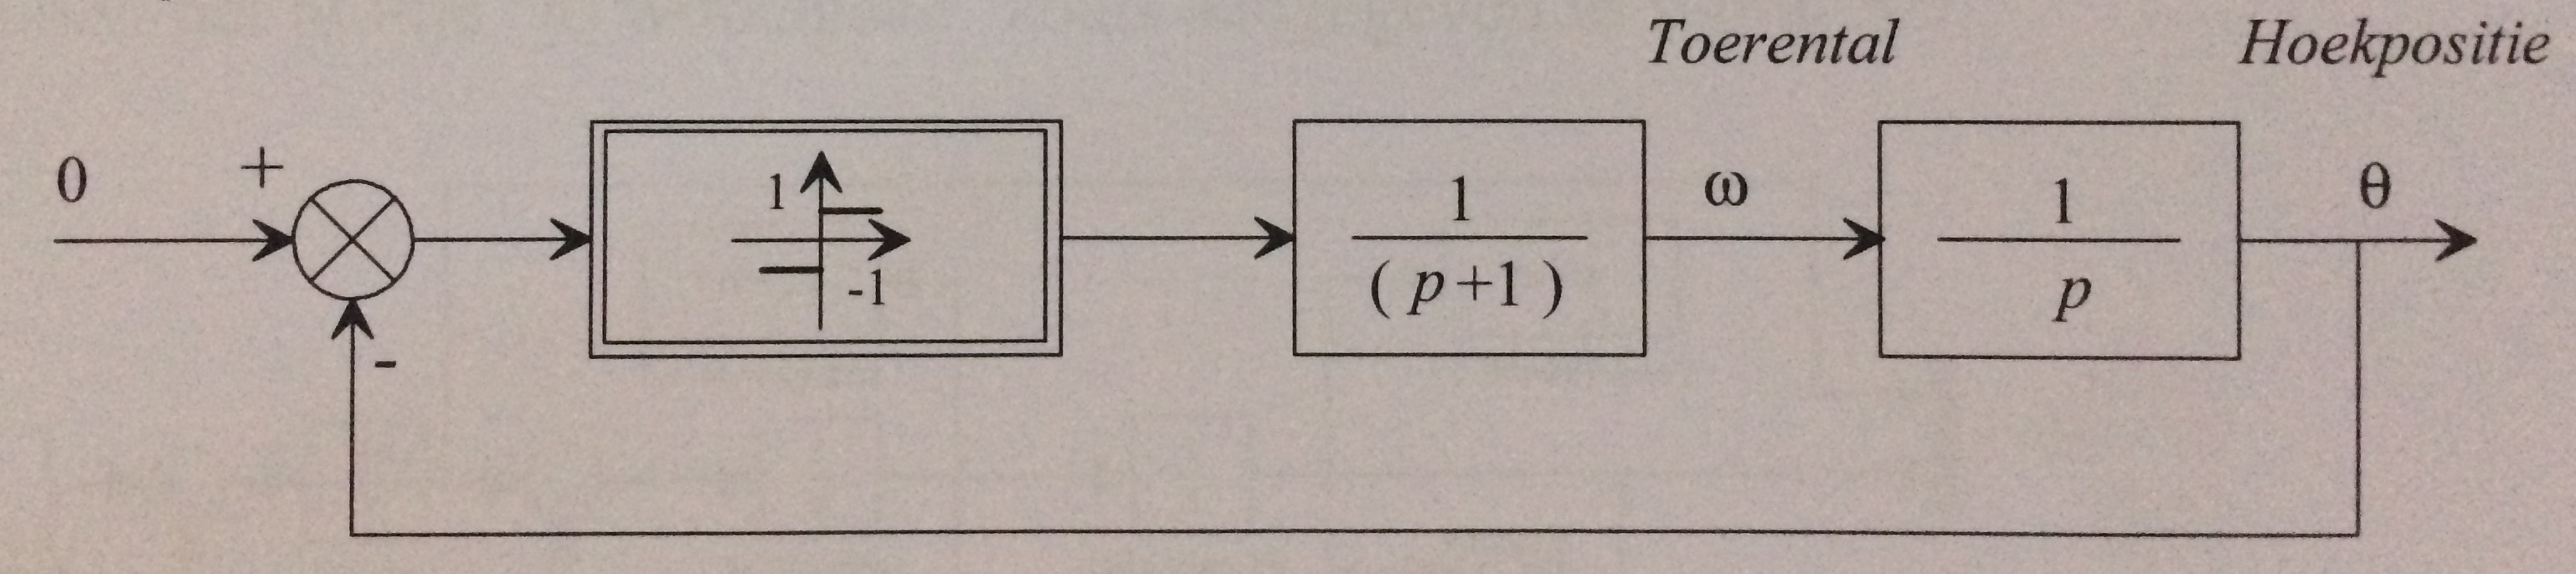
\includegraphics[width=\textwidth, keepaspectratio]{regellus.png}
	\caption{Regellus voor Aan/uit positieregeling}
	\label{regellus}	
\end{figure}

\noindent
Het niet-lineaire deel bestaat uit het aan/uit-element. Deze schakelt tussen de waarden +1 en -1 om de motor respectievelijk positief en negatief te laten draaien. De motor zelf is een eerste orde systeem met transfertfunctie $TF_{motor} = \frac{1}{p+1}$. Hieruit volgt dat $K=1$ en $\tau=1$. Gezien de hoekpositie graag gekend is wordt er tenslotte een zuivere integrator toegevoegd. Immers geldt dat $\theta = \int_{\Delta t} \omega \ \mathrm{d}t$. \\ \\
\section{Simulatie}
Om deze schakeling te simuleren in SIMULINK werd gebruik gemaakt van het schema uit figuur \ref{simulinkschema}. Deze omzetting maakt het mogelijk om de beginwaarden van $\omega$ en $\theta$ te kiezen. Als beginwaarden werden gekozen:
\[ 
\left \{
  \begin{tabular}{c}
  $\omega_0 = 2$ rad/s \\
  $\theta_0 = 1.5$ rad
  \end{tabular}
\right. 
\]
\begin{figure}[]
	\centering
	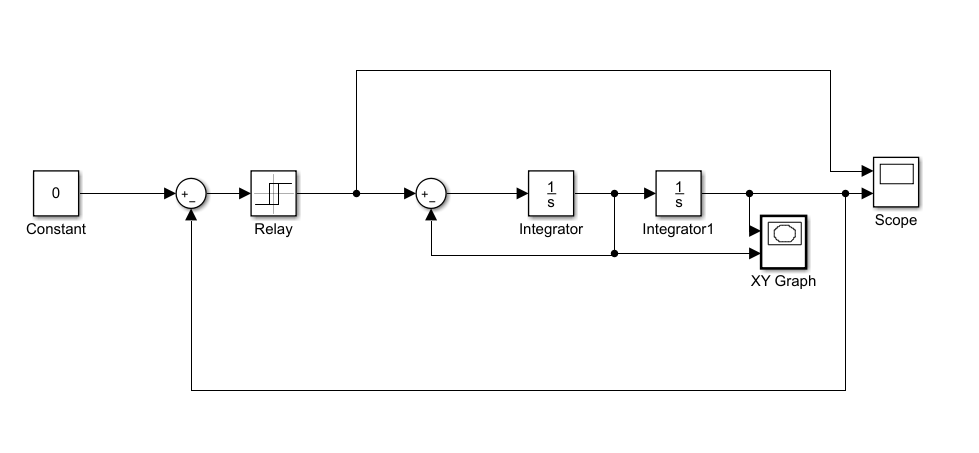
\includegraphics[width=\textwidth, keepaspectratio]{simulinkschema.png}
	\caption{Gesimuleerd schema in SIMULINK}
	\label{simulinkschema}
\end{figure}
Na een simulatie van 10 seconden levert dit de output uit figuur \ref{output1}.
\begin{figure}[]
	\centering
	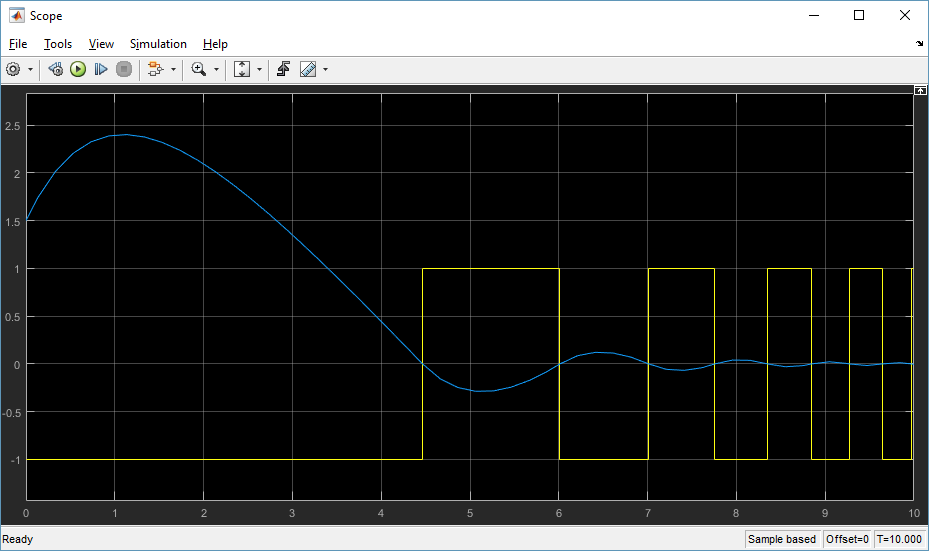
\includegraphics[width=\textwidth, keepaspectratio]{output1.png}
	\caption{Tijdrespons (10 seconden) voor $\omega_0 = 2$ rad/s en $\theta_0 = 1.5$ rad (zonder hysteresis)}
	\label{output1}
\end{figure}
\newpage
\noindent De fasetrajecten worden bepaald door $\omega$ uit te zetten als een functie van $\theta$. Deze waarden zijn rechtstreeks toegankelijk in het schema en worden geplot in een XY-grafiek. Dit levert het resultaat uit figuur \ref{xynohys}. Indien men het fasetraject wil bekomen met hysteresis dient het relais pas aan/uit te schakelen bij een bepaalde waarde. Voor figuur \ref{xyhys} werd een uit/aan-schakelwaarde van $[-0,5;0,5]$ gekozen. \\ \\

\newpage
\begin{figure}[!h]
	\centering
	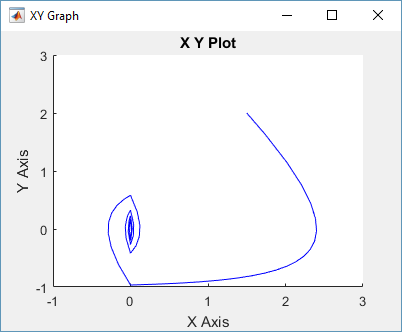
\includegraphics[height=0.4\textheight, keepaspectratio]{xynohys.png}
	\caption{Fasetraject (geen hysteresis)}
	\label{xynohys}
\end{figure}
\begin{figure}[!h]
	\centering
	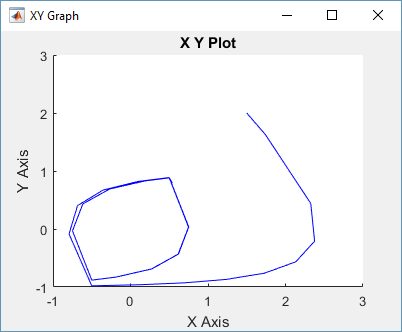
\includegraphics[height=0.4\textheight, keepaspectratio]{xyhys.png}
	\caption{Fasetraject (hysteresis)}
	\label{xyhys}
\end{figure}





\end{document}